\documentclass[12pt,titlepage]{jsarticle}
\usepackage{graphicx}
\usepackage{mediabb} %bbファイルの取得用sty

\def\maru#1{\textcircled{\scriptsize#1}}%丸囲み数字

\title{英文法の基礎\\ 論理的に英文を読む/書くために必要な知識のまとめ\\【Ver. 2012.3.3】}
\author{文責:木村修平\\Email: kimuras@fc.ritsumei.ac.jp / Twitter: @syuhei}

\begin{document}
\maketitle
\tableofcontents

\newpage


\setcounter{section}{-1}
 \section{はじめに}
 この教材は、英文法の知識に基づいて論理的に英文を読む/書くために必要な知識を、
 出来る限りわかりやすく、かつ、コンパクトにまとめたものです。

 この教材は、次のような読者を想定して作られています。
 \begin{itemize}
  \item 英語が苦手な高校生
  \item 英語が苦手な大学生、特に受験科目で英語を勉強せずに入学した大学生
  \item 英語によるコミュニケーションは問題ないけれど、文法知識に自信のない帰国子女
  \item 英語の勉強をやり直したい社会人
 \end{itemize}

   \subsubsection*{【この教材を利用したい英語教員の方へ】}
   もし英語教員の方などでこの教材をご自身の授業で使いたいという方がおられましたら、どうぞご自由にご利用ください。
   内容の加筆・改変はもちろん、再配布もご自由に行なっていただいて構いません。
   この教材は、「クリエイティブ・コモンズ 表示 - 非営利 - 継承 2.1 日本 ライセンス」の下に提供されています。
   この教材の電子データ(Word形式・PDF形式)の入手およびライセンスの詳細につきましては、下記URLをご覧ください。

   【Mt. English Project:http://mep.papiko.com/】


 \section{語と品詞}
 ここでは、英文に含まれている語と品詞の関係について説明します。
 
 英語で書かれた文を{\bf 英文}と呼びます。英文は複数の{\bf 語}(=単語)によって形作られています。
 たとえば次の英文は4つの語で成り立っています(図 \ref{fig1})。

 
 \begin{figure}[htbp]
  \begin{center}
   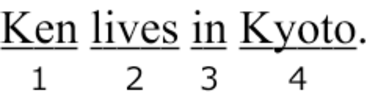
\includegraphics[width=5cm]{./figure/fig1.pdf}
   \caption{4つの語で作られた英文}
   \label{fig1}
  \end{center}
 \end{figure}
 
 英文に含まれるすべての語は何らかの{\bf 品詞}に分類することができます。
 語と品詞の関係は、コンビニで売られている商品とその裏側に記載されているバーコードとの関係に似ています。
 つまり、コンビニの商品のひとつひとつにバーコードがくっついているように、英文の中の語のひとつひとつに品詞というバーコードがついているのです。

 先ほどの英文に含まれる語をひっくり返して品詞=バーコードを確認してみましょう(図 \ref{fig2})。

 \begin{figure}[htbp]
  \begin{center}
   
\includegraphics[width=5cm]{./figure/fig2.pdf}
   \caption{4つの語で作られた英文}
   \label{fig2}
  \end{center}
 \end{figure}


 それぞれの語の品詞を確認してみると、Kenには「人やモノを意味するバーコード」である{\bf 名詞}が、livesには「動作を表すバーコード」である{\bf 動詞}が、inには「場所や時間を表すバーコード」である{\bf 前置詞}が、そしてKyotoには{\bf 名詞}というバーコードがくっついていることがわかります。
 このように、英文の中の語はすべて何らかの品詞に分類できます。
 論理的に英文を読む/書くためには、英文を品詞のレベルでとらえる必要があります。
 そのためには英文法の知識が必要です。
 そして、{\bf 英文法とは品詞レベルのルールの集まり}のことなのです。

 では、品詞にはいくつの種類があるのでしょうか。
 英文を構成する主な品詞は次の13種類です。

 \begin{enumerate}
  \item 名詞(Noun / n.)
  \item 代名詞(Pronoun / pron.)
  \item 形容詞(Adjective / adj. / a.)
  \item 副詞(Adverb / adv. / ad.)
  \item 動詞(Verb / v.)
  \item 前置詞(Preposition / prep.)
  \item 接続詞(Conjunction / conj.)
  \item 間投詞(Interjection / interj. / int.)
  \item 助動詞(Auxiliary / aux.)
  \item 冠詞(Article / art.)
  \item 動名詞(Gerund / ger.)
  \item 不定詞(Infinitive / infin. / inf.)
  \item 分詞(Participle / part. / p.)
 \end{enumerate}
 

 品詞の名前を今すべて覚える必要はありません。
 ここで理解するべきは、{\bf 英文は、これら13の主要な品詞が組み合わさって出来ている}ということです。
 辞書で語の意味を調べるときには、{\bf 意味だけでなく品詞にも注目する習慣}をつけてください(図 \ref{fig3})。
  \begin{figure}[htbp]
   \begin{center}
    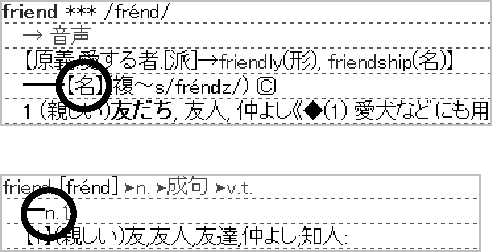
\includegraphics[width=7cm]{./figure/fig3.pdf}
    \caption{辞書で語の意味を引くときは品詞情報にも注目}
    \label{fig3}
   \end{center}
  \end{figure}


 \section{品詞と文の要素}
 ここでは、品詞と文の要素の対応関係について説明します。

 英文を品詞レベルで考えることがなぜそれほど大切なのでしょうか?
 それは、{\bf 品詞の種類によって英文の中で果たす役割が決まる}からです。
 「役割」の中でも、主語(S)・述語動詞(V)・目的語(O)・補語(C)という特に大切な4つの役割を、まとめて{\bf 文の要素}と呼びます。

 品詞と文の要素のあいだには次の対応関係が存在しています(表\ref{tab1})。
 \begin{table}[htbp]
  \begin{center}
   \caption{品詞と文の要素の対応関係}
   \begin{tabular}{|c|ll|}
    \hline
    品詞 & \multicolumn{2}{|c|}{文の要素} \\ \hline \hline
    名詞 & 主語 & ({\bf S}ubject) \\ 
    & 目的語 & ({\bf O}bject) \\
    & 補語 & ({\bf C}omplement) \\ \hline
    動詞 & 述語動詞 & ({\bf V}erb) \\ \hline
    形容詞など & 補語 & ({\bf C}omplement) \\ \hline
   \end{tabular}
   \label{tab1}
  \end{center}
 \end{table}
 つまり、もしある語が名詞である場合、その語は英文の中でS / O / Cという文の要素の役割を担っている可能性があるということです。
 先ほどの例文で出てきたKen(ケン)という人名は名詞ですから、S / O / Cの役割になれるのです。
 Cの役割になれる品詞は上の表では名詞と形容詞だけですが、他にも、不定詞や分詞などもCの役割をする可能性があります。
 ただ、現時点では最低限、上の表をしっかり覚えておくだけで十分です。


 \section{語と句と節}
 ここでは、語と句と節という文法用語について解説します。
 
 語と句と節という用語は、英文の構造を論理的に考えるときの大切な区切りの単位です。
 今後の学習の過程で頻繁に出てくる用語ですので、曖昧なままにしないでおきましょう。

 語というのは、ひとつの単語のことです。
 次のcar(車)というひとつの単語は、前後に他の語がくっついていませんので、語と呼びます(図\ref{fig4})。
  \begin{figure}[htbp]
   \begin{center}
    
\includegraphics[width=2cm]{./figure/fig4.pdf}
    \caption{語の例}
    \label{fig4}
   \end{center}
  \end{figure}

  句というのは、複数の語がくっついて一つのかたまりになっているものです。
  次のmy car(私の車)はmyという語とcarという語がくっついて一つの意味を成していますので、句と言えます(図\ref{fig5})。
  \begin{figure}[htbp]
   \begin{center}
    
\includegraphics[width=3cm]{./figure/fig5.pdf}
    \caption{句の例}
    \label{fig5}
   \end{center}
  \end{figure}


  節というのは、複数の語がくっついて一つのかたまりになっており、かつ、その中に主語(S)と述語(V)が存在しているかたまりを指します(図\ref{fig6})。
  \begin{figure}[htbp]
   \begin{center}
    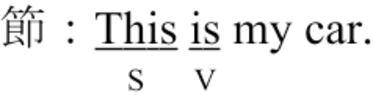
\includegraphics[width=4cm]{./figure/fig6.pdf}
    \caption{節の例。節にはSとVが含まれる}
    \label{fig6}
   \end{center}
  \end{figure}


  節という文法用語を平易なことばに直すと{\bf 文}になります。
  つまり、1. 語と品詞で「英語で書かれた文を英文と呼ぶ」と書きましたが、文=節にはSとVが含まれている必要がありますので、carのような語やmy carのような句は、厳密に言いますと、英文とは呼べないということになります。

  \newpage
 \section{自動詞と他動詞}
 ここでは、英語の動詞の分類について、自動詞と他動詞を中心に解説します。
 自動詞と他動詞の違いをきちんと理解することは、次章で述べる五文型の知識に繋がります。

 英文を成り立たせているのは13個の品詞だと先に述べました。
 その中でも、英文を成り立たせる上で最も重要な品詞が動詞です。
 英文の中で動詞がどのような役割を果たしているのかがわからなければ英文を論理的に読めませんし、自分でもまともな英文を書くことはできないでしょう。
 言い方を変えれば、{\bf 動詞の理解を深めておけば正しく英文を読める/書ける可能性が飛躍的に高まる}のです。

 まず、英語の動詞の基本的な知識を身につけましょう。
 ここでは、英語を{\bf 自動詞}と{\bf 他動詞}に分けて考えることから始めます。
 {\bf 自動詞と他動詞の違いは、動詞として意味が成り立つために動詞の後ろに目的語(O)を必要とするか、必要としないか}です(図\ref{fig7})。
  \begin{figure}[htbp]
   \begin{center}
    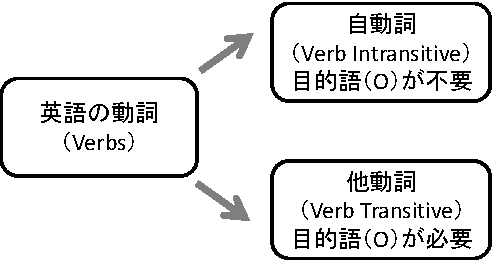
\includegraphics[width=8cm]{./figure/fig7.pdf}
    \caption{英語の動詞は自動詞と他動詞に分かれる}
    \label{fig7}
   \end{center}
  \end{figure}

  ここで、品詞と文の要素の対応関係を思い出してください。
  目的語(O)になれる品詞は名詞だけです。
  ですから、もしある動詞が自動詞である場合、その後ろには目的語(O)としての名詞が無いはずです(補語Cとしての名詞はあるかもしれません)。
  もしある動詞が他動詞の場合、その後ろには目的語(O)としての名詞が必ず存在するはずです。

  たとえば、動詞discussを辞書で引いてみて下さい。
  一般的な学習者向け辞書(大修館書店『ジーニアス英和辞典 第4版』など)では、discussは他動詞として登録されているはずです。
  他動詞であれば、「他」や「v.t.」(Verb Transitiveの略)などと略記されています(図\ref{fig8})。
  \begin{figure}[htbp]
   \begin{center}
    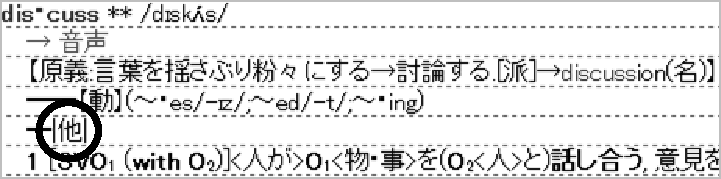
\includegraphics[width=8cm]{./figure/fig8.pdf}
    \caption{『ジーニアス英和辞典』のdiscussの項目}
    \label{fig8}
   \end{center}
  \end{figure}

いま確認したとおりdiscussは他動詞ですから、たとえばdiscussを含む次のような英文を品詞レベルで解析すると、図\ref{fig9}のようになります(冠詞のtheはproblemと一緒に扱っています)。
  \begin{figure}[htbp]
   \begin{center}
    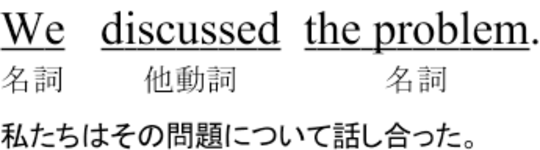
\includegraphics[width=8cm]{./figure/fig9.pdf}
    \caption{discussを含む英文を品詞レベルで解析}
    \label{fig9}
   \end{center}
  \end{figure}

  次に、それぞれの品詞がどの文の要素と対応しているのかを考えてみますと、図\ref{fig10}になります。
  \begin{figure}[htbp]
   \begin{center}
    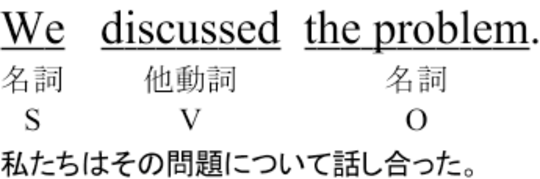
\includegraphics[width=8cm]{./figure/fig10.pdf}
    \caption{discussを含む英文の品詞と文の要素の対応関係}
    \label{fig10}
   \end{center}
  \end{figure}

  S+V+Oというのは次章で解説する五文型の中の第3文型にあたります。
  discussという動詞が他動詞であることがわかれば、文型を論理的に特定することができます。

  英語の動詞には、is / am / areなどのような{\bf be動詞}と、be動詞以外の(discussのような){\bf 一般動詞}が存在します。
  一般動詞の多くには自動詞と他動詞両方の使い方がありますが、be動詞には自動詞としての使い方しかありません。
  自動詞と他動詞、be動詞と一般動詞の関係、そしてbe動詞と一般動詞それぞれが取れる文型の可能性をまとめたのが図\ref{fig11}になります。
  文型については次章で解説します。
  \begin{figure}[htbp]
   \begin{center}
    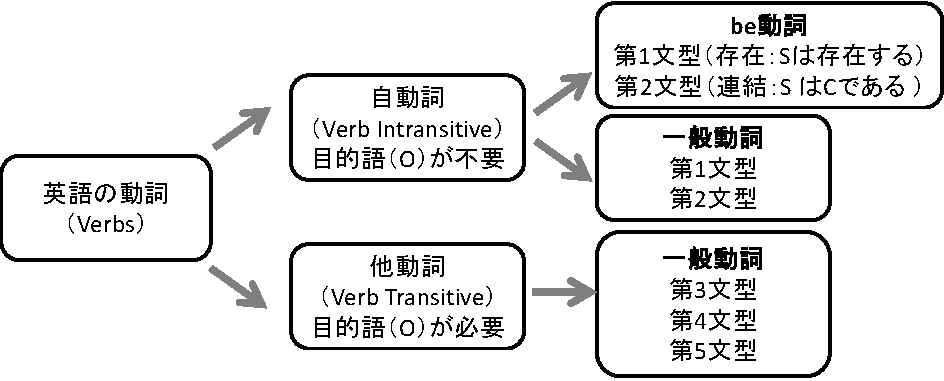
\includegraphics[width=8cm]{./figure/fig11.pdf}
    \caption{自動詞と他動詞、be動詞と一般動詞の関係}
    \label{fig11}
   \end{center}
  \end{figure}


  \section{五文型を使った英文の分類}
  ここでは、英文を5つのパターンに分類する五文型の考え方を解説します。
  五文型というアイデアは、イギリスの英語学者・C. T. Onions(1873-1965)の考えに由来しています(An Advanced English Syntaxという本の中のForms of the Predicate)。

  ある英文が5つのパターンの中のどれに当てはまるのかはその英文の中の動詞の型番によって決まります。
  ですからこのテキストでは、動詞部分を単に「V」(Verbの略)と書くのではなく、動詞の型番を数字で書いて丸囲みすることによってその動詞が何番の文型をつくっているのかを、これ以降は明示することにします。
たとえば図\ref{fig12}は動詞が\maru{3}と書かれていますので第3文型であることを意味します。
  \begin{figure}[htbp]
   \begin{center}
    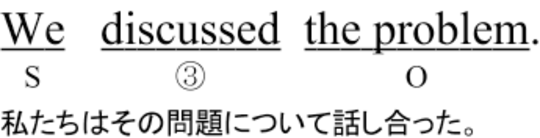
\includegraphics[width=8cm]{./figure/fig12.pdf}
    \caption{第3文型の例}
    \label{fig12}
   \end{center}
  \end{figure}

  五文型を使うメリットには、英文をパターン化できるということの他に、日本語訳もある程度パターン化できるという点があります。
  先ほどの英文ですと、第3文型ですから、まず「Weはthe problemをdiscussした」という訳のパターンにはめこみ、そのあとで微調整をすればよいのです。
  以下の表\ref{tab2}は、5つの文型についてまとめたものです。
 \begin{table}[htbp]
  \begin{center}
   \caption{五文型の一覧}
   \begin{tabular}{|c|c|c|c|}
    \hline
    文型 & 文の要素 & 使われる動詞 & 例文と特徴 \\ \hline \hline
    {\bf 第1文型} & S \maru{1} & \shortstack{be動詞(存在:Sは存在する)\\自動詞(完全自動詞)} & \shortstack {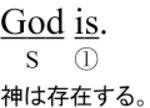
\includegraphics[width=2cm]{./figure/tab2_1.pdf} \\ 修飾語句を伴うことが多い}
 \\\hline
    \multicolumn{4}{|c|}{日本語訳の例:Sは\maru{1}する。}\\ \hline

    {\bf 第2文型} & S \maru{2} C & \shortstack{be動詞(存在:Sは存在する)\\自動詞(完全自動詞)} & \shortstack {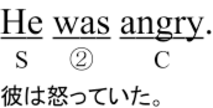
\includegraphics[width=4cm]{./figure/tab2_2.pdf} \\ C の意味上の主語=S}
 \\\hline
    \multicolumn{4}{|c|}{日本語訳の例:SはC[である。/になる。/に見える。]など}\\ \hline

    {\bf 第3文型} & S \maru{3} O & 他動詞(完全他動詞) & 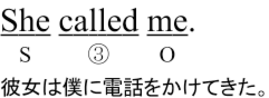
\includegraphics[width=5cm]{./figure/tab2_3.pdf} \\\hline
    \multicolumn{4}{|c|}{日本語訳の例:SはOを\maru{3}する。}\\ \hline

    {\bf 第4文型} & S \maru{4} O1 O2 & \shortstack{他動詞(完全他動詞)\\【授与/剥奪の意味が多い】} & \shortstack {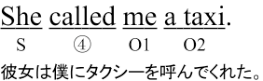
\includegraphics[width=5cm]{./figure/tab2_4.pdf} \\ S\maru{3}Oに書換え可能\\(できないものもある)}
 \\\hline
    \multicolumn{4}{|c|}{日本語訳の例:SはO1にO2を\maru{4}する。(授与)/O1からO2を\maru{4}する。(剥奪)}\\ \hline

    {\bf 第5文型} & S \maru{5} O C & 他動詞(不完全他動詞) & \shortstack {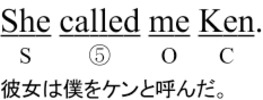
\includegraphics[width=5cm]{./figure/tab2_5.pdf} \\ C の意味上の主語=O}

 \\\hline
    \multicolumn{4}{|c|}{日本語訳の例:SはO をC(の状態になることや動作をすること)に\maru{5}する。}\\ \hline

   \end{tabular}
   \label{tab2}
  \end{center}
 \end{table}


 \section{修飾関係の基礎}
 ここでは、修飾関係について、その基本的な原理を解説します。
 
 {\bf 修飾}(Modification)とは、{\bf あることばが別のことばを説明する関係}のことです。日本語を例に修飾関係を考えてみますと、たとえば、「ブリキ製のおもちゃの赤い車」という語句の中には、次のような説明する/説明されるの関係が成り立っていることがわかります(図\ref{fig13})。
  \begin{figure}[htbp]
   \begin{center}
    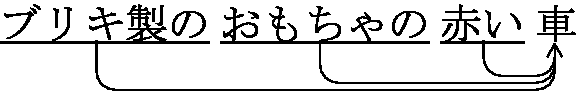
\includegraphics[width=8cm]{./figure/fig13.pdf}
    \caption{日本語の修飾関係の例}
    \label{fig13}
   \end{center}
  \end{figure}
 
 どのことばが別のどのことばを修飾するのかは、品詞レベルで対応関係が決まっています。
 つまり、{\bf 説明する品詞と説明される品詞のあいだの対応関係にはルールが存在する}のです。
 英語の場合ですと、修飾する品詞と修飾される品詞の対応関係は表\ref{tab3}になります。
 \begin{table}[htbp]
  \begin{center}
   \caption{修飾関係の品詞ごとの対応}
   \begin{tabular}{|c|c|c|}
    \hline
    修飾する品詞 & 修飾される品詞 & 例 \\ \hline \hline
    形容詞(句/節) & 名詞 & 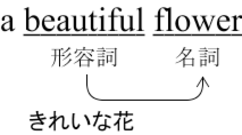
\includegraphics[width=3cm]{./figure/tab3_1.pdf} \\
    \hline
    & 動詞 & 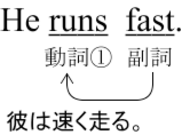
\includegraphics[width=3cm]{./figure/tab3_2.pdf} \\ \cline{2-3}
    副詞(句/節)& 形容詞 & 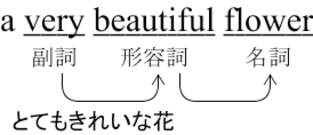
\includegraphics[width=4cm]{./figure/tab3_3.pdf} \\ \cline{2-3}
    & 副詞 & 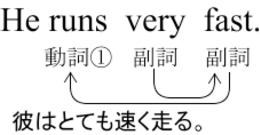
\includegraphics[width=4cm]{./figure/tab3_4.pdf} \\ \hline
   \end{tabular}
   \label{tab3}
  \end{center}
 \end{table}


 \section{前置詞+名詞による形容詞句と副詞句}
 ここでは、前置詞と名詞の組み合わせが形容詞句と副詞句になることを解説します。
 
 in, at, for, to, of, fromなどの単語は前置詞という品詞に分類されます。
 前置詞のうしろには名詞が置かれる可能性が高く、そのため英文の中では{\bf 前置詞+名詞のセット}で登場します。

 前置詞と名詞がセットになると、形容詞句または副詞句の働きをします。
 どちらも句ですから、2語(前置詞+名詞)以上の組み合わせで、その中にS+V(節)がありません。

 句という言葉がつくと難しく聞こえますが、形容詞句とは句のかたちをして形容詞の働きをする(Cになるか、または名詞を修飾する)かたまり、副詞句は句のかたちをして副詞の働きをする(動詞/形容詞/副詞を修飾する)かたまりのことです(図\ref{fig14})。
  \begin{figure}[htbp]
   \begin{center}
    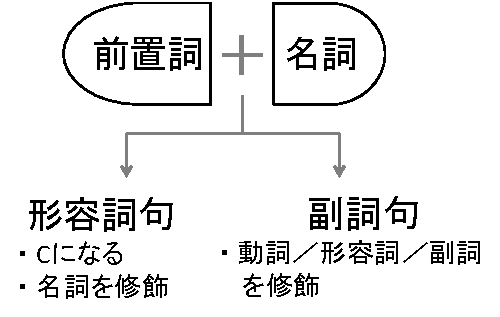
\includegraphics[width=8cm]{./figure/fig14.pdf}
    \caption{前置詞+名詞の働き}
    \label{fig14}
   \end{center}
  \end{figure}

  英文内の語句が形容詞の働きをしている場合は丸括弧( )で、副詞の働きをしている場合は< >でくくると英文の構造が見やすくなります(図\ref{fig15})。
  \begin{figure}[htbp]
   \begin{center}
    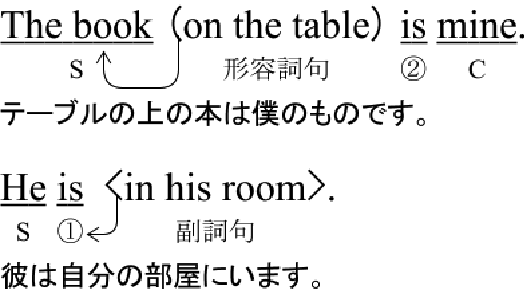
\includegraphics[width=8cm]{./figure/fig15.pdf}
    \caption{形容詞句と副詞句の例}
    \label{fig15}
   \end{center}
  \end{figure}

  注目してほしいのは、どちらの英文でも形容詞句と副詞句は修飾する側の語句として働いています。
  修飾語句というのは「飾り」ですから、{\bf 修飾語句である形容詞句と副詞句を取り外しても文型には影響しません。}

  \newpage
  \section{最終チェック}
  次の各英文を、これまでに学んだ知識に基づいて構造(文型と修飾関係)を解析し、さらに和訳しましょう。
 \begin{table}[htbp]
    \begin{tabular}{ll}
     (1) & Tom lives in Kyoto. \\
     & He is a teacher of English. \\
     & He teaches at two different schools.\\
     (2) & Ken married Aki in 1998.\\
     & She worked at a bookstore across his office.\\
     & They first met in 1996.\\
     (3) & Father bought me a dog when I was young.\\
     & I named the dog Lucky.\\
     & He was my best friend.\\
     (4) & My mother often read me a story at my bedside when I was young.\\
     (5) & Every second counts.\\
     (6) & She made herself at home in her room.\\
     (7) & There are many Chinese restaurants in this city.\\
    \end{tabular}
 \end{table}


 \section{付録:英語学習を助ける道具たち}
 \subsection*{辞書}
  \begin{itemize}
   \item 辞書は{\bf 最強の単語帳}
   \item 辞書で語の意味を引くときには、必ず{\bf 品詞情報を先に見る癖}をつける
   \item 主な英和辞書
         \begin{itemize}
          \item ジーニアス英和辞典(大修館書店)
          \item ジーニアス和英辞典(大修館書店)
          \item ジーニアス大英和辞典(大修館書店)
          \item リーダーズ英和中辞典(研究社)
          \item リーダーズ和英中辞典(研究社)
          \item プログレッシブ英和中辞典(小学館)
          \item プログレッシブ和英中辞典(小学館)
          \item ウィズダム英和辞典(三省堂)
          \item コウビルド英英辞典(紀伊国屋書店)
          \item ロングマン現代英英辞典(桐原書店)
          \item オックスフォード現代英英辞典(増進会出版)
          \item クラウン受験英語辞典(三省堂)
         \end{itemize}
   \item \underline{使い方を誤らなければ}{\bf 電子辞書}はとても便利
   \item 表示領域が極端に狭い電子辞書は不可
   \item 電子辞書購入の際の注意点
         \begin{itemize}
          \item 店頭で実機を触ってみる
          \item 起動時間を計測する
          \item 価格.com(kakaku.com)で最安値情報をチェック
          \item 本体に氏名と連絡先を記入する
          \item レシートおよび保証書は大切に保管する
         \end{itemize}
  \end{itemize}

  \subsection*{参考書A(基礎)}
  \begin{itemize}
   \item 参考書Aは基礎レベルに対応
   \item イラスト入りのものが多く、初学者にやさしい
   \item 主な参考書A
         \begin{itemize}
          \item ラーナーズ高校英語(数研出版)
          \item 総合英語 Forest(桐原書店)
          \item デュアルスコープ総合英語(数研出版)
          \item 安河内の「はじめてわかる」英文法(三省堂)
         \end{itemize}
  \end{itemize}

  \subsection*{参考書B(発展)}
  \begin{itemize}
   \item 学習を進めると、必ず参考書Aでは限界が出てくる
   \item 参考書Bは発展レベルに対応
   \item 文字ばかりで最初は抵抗があるかもしれないが、使いこなせれば強力な相棒になる
   \item 主な参考書B
         \begin{itemize}
          \item 表現のためのロイヤル英文法(旺文社)
          \item depth 英語総合(河合出版)
          \item 英文法詳解(学習研究社)
          \item ロイヤル英文法(旺文社)
          \item 英文法解説(金子書房)
          \item 英文法総覧(開拓社)
          \item 現代英文法講義(開拓社)
         \end{itemize}
  \end{itemize}
  \subsection*{Mt. English Project の宣伝}
  \begin{itemize}
   \item Mt. English Grammar(Mt. English Project内):http://mep.papiko.com/
         \begin{itemize}
          \item 自由に使えるオンライン英文法参考書(作成途中ですが・・・)
         \end{itemize}
  \end{itemize}
\end{document}
